\documentclass[12pt]{article}
\usepackage[dvipsnames]{xcolor}
\usepackage{graphicx}
\usepackage{amsmath}
\usepackage{amssymb}
\usepackage[color,matrix,frame,arrow,curve]{xy}
\begin{document}


\begin{figure}[h!]\centering
\begin{minipage}{.5\linewidth}
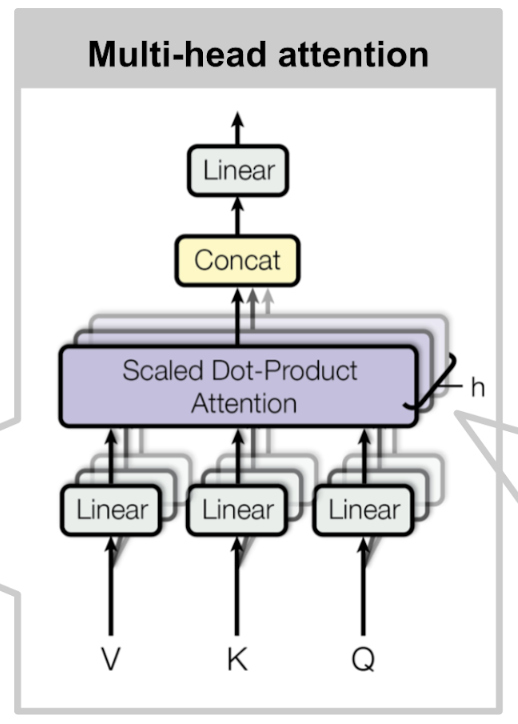
\includegraphics[width=2in]{multi-head-att.jpg}
\end{minipage}%blank lines between minispaces breaks this
\begin{minipage}{.5\linewidth}
$$\xymatrix{
&*+[F*:SpringGreen]{\underline{1}^{3\times  4}}\ar[dr]\ar[ddddr]\ar[dddddddr]&&&
\\
*+[F*:Dandelion]{\underline{Q}^{3\times  4}}\ar[ur]\ar[r]\ar[dr]&*+[F*:SpringGreen]{\underline{2}^{3\times  4}}\ar[r]\ar[dddr]\ar[ddddddr]&*+[F*:Orchid]{\underline{X}^{3\times  4}}\ar[dddr]&&
\\
&*+[F*:SpringGreen]{\underline{3}^{3\times  4}}\ar[ur]\ar[ddr]\ar[dddddr]&&&
\\
&*+[F*:SpringGreen]{\underline{4}^{3\times  4}}\ar[uur]\ar[dr]\ar[ddddr]&&&
\\
*+[F*:Dandelion]{\underline{K}^{3\times  4}}\ar[ur]\ar[r]\ar[dr]&*+[F*:SpringGreen]{\underline{5}^{3\times  4}}\ar[uuur]\ar[r]\ar[dddr]&*+[F*:Orchid]{\underline{Y}^{3\times  4}}\ar[r]&*+[F*:yellow]{\underline{C}^{3\times  4}}\ar[r]&*+[F*:SpringGreen]{\underline{L}^{3\times  4}}
\\
&*+[F*:SpringGreen]{\underline{6}^{3\times  4}}\ar[uuuur]\ar[ur]\ar[ddr]&&&
\\
&*+[F*:SpringGreen]{\underline{7}^{3\times  4}}\ar[uuuuur]\ar[uur]\ar[dr]&&&
\\
*+[F*:Dandelion]{\underline{V}^{3\times  4}}\ar[ur]\ar[r]\ar[dr]&*+[F*:SpringGreen]{\underline{8}^{3\times  4}}\ar[uuuuuur]\ar[uuur]\ar[r]&*+[F*:Orchid]{\underline{Z}^{3\times  4}}\ar[uuur]&&
\\
&*+[F*:SpringGreen]{\underline{9}^{3\times  4}}\ar[uuuuuuur]\ar[uuuur]\ar[ur]&&&
}$$
\end{minipage}
\caption{Multi-head Attention.}
\label{fig-texnn-for-multi-head-att}
\end{figure}\begin{subequations}
\begin{equation}
Q^{3\times  4} =)
\label{eq-Q-fun-multi-head-att}
\end{equation}

\begin{equation}
K^{3\times  4} =)
\label{eq-K-fun-multi-head-att}
\end{equation}

\begin{equation}
V^{3\times  4} =)
\label{eq-V-fun-multi-head-att}
\end{equation}

\begin{equation}
1^{3\times  4} = {\rm linear}(Q^{3\times  4})
\label{eq-1-fun-multi-head-att}
\end{equation}

\begin{equation}
2^{3\times  4} = {\rm linear}(Q^{3\times  4})
\label{eq-2-fun-multi-head-att}
\end{equation}

\begin{equation}
3^{3\times  4} = {\rm linear}(Q^{3\times  4})
\label{eq-3-fun-multi-head-att}
\end{equation}

\begin{equation}
4^{3\times  4} = {\rm linear}(K^{3\times  4})
\label{eq-4-fun-multi-head-att}
\end{equation}

\begin{equation}
5^{3\times  4} = {\rm linear}(K^{3\times  4})
\label{eq-5-fun-multi-head-att}
\end{equation}

\begin{equation}
6^{3\times  4} = {\rm linear}(K^{3\times  4})
\label{eq-6-fun-multi-head-att}
\end{equation}

\begin{equation}
7^{3\times  4} = {\rm linear}(V^{3\times  4})
\label{eq-7-fun-multi-head-att}
\end{equation}

\begin{equation}
8^{3\times  4} = {\rm linear}(V^{3\times  4})
\label{eq-8-fun-multi-head-att}
\end{equation}

\begin{equation}
9^{3\times  4} = {\rm linear}(V^{3\times  4})
\label{eq-9-fun-multi-head-att}
\end{equation}

\begin{equation}
X^{3\times  4} = {\rm scaled\_dot\_prod\_att}(1^{3\times  4},2^{3\times  4},3^{3\times  4},4^{3\times  4},5^{3\times  4},6^{3\times  4},7^{3\times  4},8^{3\times  4},9^{3\times  4})
\label{eq-X-fun-multi-head-att}
\end{equation}

\begin{equation}
Y^{3\times  4} = {\rm scaled\_dot\_prod\_att}(1^{3\times  4},2^{3\times  4},3^{3\times  4},4^{3\times  4},5^{3\times  4},6^{3\times  4},7^{3\times  4},8^{3\times  4},9^{3\times  4})
\label{eq-Y-fun-multi-head-att}
\end{equation}

\begin{equation}
Z^{3\times  4} = {\rm scaled\_dot\_prod\_att}(1^{3\times  4},2^{3\times  4},3^{3\times  4},4^{3\times  4},5^{3\times  4},6^{3\times  4},7^{3\times  4},8^{3\times  4},9^{3\times  4})
\label{eq-Z-fun-multi-head-att}
\end{equation}

\begin{equation}
C^{3\times  4} = {\rm concat}(X^{3\times  4},Y^{3\times  4},Z^{3\times  4})
\label{eq-C-fun-multi-head-att}
\end{equation}

\begin{equation}
L^{3\times  4} = {\rm concat}(C^{3\times  4})
\label{eq-L-fun-multi-head-att}
\end{equation}

\end{subequations}


\end{document}  
